\chapter{Opis projektu}
\section{Opis}
W poprzednich rozdziałach zostały przedstawione metody klastrowania oraz zarządzania konfiguracją, a następnie zostały one przetestowane.
Została również wykazana zasadność ich stosowania.\\
Jednak, aby wdrożyć takie rozwiązania, potrzebna jest wiedza oraz czas pracy administratora.

\textit{System zautomatyzowanego zarządzania konfiguracją farmy serwerów aplikacji WWW} (zwany dalej \textit{SZZ}) ma za zadanie uprościć konfigurację klastra WWW, pozwalając zaoszczędzić czas i pieniądze.
Opisywany system będzie mógł być obsługiwany przez osoby nie posiadające dogłębnej wiedzy z zakresu administracji systemami linux ani serwerami WWW.
Wymagana jest jedynie podstawowa wiedza techniczna, którą posiada przeciętny programista.

Konfiguracja odbywa się poprzez edycję plików, dlatego obsługująca system powinna być w stanie obsługiwać połączenia \texttt{ssh} oraz edytor tekstowy.
\section{Struktura}
\textit{SZZ} wykorzystuje różne metody klastrowania.
Struktura systemu została przedstawiona na rys~\ref{fig:struktura}
\begin{figure}
	\centering
	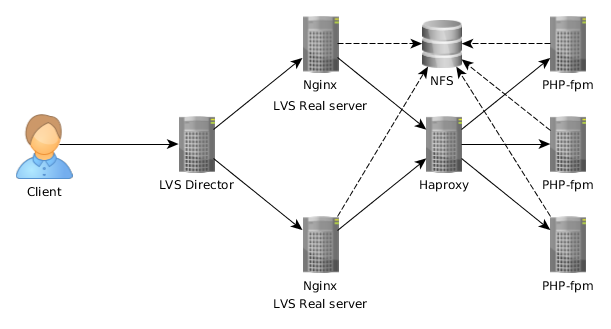
\includegraphics[width=\textwidth]{obrazy/struktura_szz.png}
	\caption{Struktura SZZ}
	\label{fig:struktura}
\end{figure}
Pierwszą warstwą klastrowania jest LVS (por.~\ref{sec:LVS}).
Zapytanie trafiające na serwer obsługiwane są przez \textit{direcotor}-a.
Następnie przekazywane są do serwerów WWW, które analizując zapytania serwują treści statyczne ze wspólnego zasobu NFS.
W przypadku zapytania o treści dynamiczne, zapytania przekazywane jest do warstwy trzeciej projektu, czyli usługi Haproxy, która przekazuje zadania do odpowiedniego serwera z usługą \textit{PHP-fpm}.
Po wygenerowaniu odpowiedzi, serwer roboczy zwraca odpowiedź do Haproxy, które przekazuje je do serwera WWW.
Ten natomiast, będąc \textit{real server}-em w klastrze LVS, odpowiada bezpośrednio klientowi.
\subsection{Warstwa zero - storage}
Projekt posiada wspólny zasób dyskowy wystawiany poprzez protokół NFS.
Metoda ta w znaczny sposób uprasza aktualizację aplikacji na wszystkich węzłach równocześnie - kosztem braku możliwości wykonywania tzw. \textit{rolling update}.
Ta technologia rozwiązuje również problem wgrywania plików na serwer oraz ich propagacji, ponieważ każdy wgrywany plik trafia na wspólny zasób i jest od razu widziany przez pozostałe węzły.\\
Wydajność NFS jest zadowalająca przy wykorzystywaniu w obrębie jeden serwerowni i jednej sieci LAN.
W przypadku chęci użycia rozproszenia systemu między kilkoma \textit{datacenter} należy ze własnym zakresie obsłużyć synchronizację wgrywanych plików oraz aktualizacji.
\subsection{Warstwa pierwsza - LVS}
Jedynym wystawionym na świat serwerem jest \textit{director}. Do niego trafiają wszystkie zapytania od klientów.
Wykorzystana w projekcie konfiguracja używa \textit{scheduler}-a opartego o algorytm \textit{round robin}, czyli przekazuje zapytania na wszystkie serwery po kolei.
Technologia LVS pozwala na posiadanie tylko jednego serwera typu \textit{director}, ponieważ jego zadaniem jest jedynie przekazywanie zapytać do \textit{real server}-ów.
Ponadto, jak zostało omówione wcześniej, odpowiedzi do klienta wysyłane są bezpośrednio od \textit{real server}-ów, bez udziału \textit{director}-a co pozwala na obsługę nawet dużego ruchu.\\
Obecna konfiguracja nie posiada narzędzi do wykrywania niedostępności \textit{director}-a bądź \textit{real server}-ów, dlatego konfiguracja narzędzi typu \textit{heartbeat} oraz technologii  \textit{floating IP} i/lub monitoringu stanu serwerów, leży po stronie użytkownika.
\subsection{Warstwa druga - Nginx}
Drugą warstwą jest warstwa serwerów WWW.
Do nich trafiają zapytania przekazywane z pierwszej warstwy.
Serwer WWW obsługujący wiele \textit{Virtual Host}-ów, analizuje zapytanie pod kontem, czy żądana ścieżka jest istniejącym plikiem na dysku.
Jeżeli plik istnieje, jest on serwowany klientowi.
W przeciwnym wypadku, zapytanie zostaje przekazywane do haproxy.
\subsection{Warstwa trzecia - Haproxy}
Haproxy jest trzecią warstwą systemu.
Przez tą warstwę przechodzą wszystkie zapytania o treści dynamiczne.
Usługa tworzy osobny \textit{frontend} oraz \textit{backend} dla każdego projektu.\\
Haproxy posiada wbudowaną obsługę wykrywania, dlatego warstwa trzecia zapewnia pełna \textit{HA}.\\
Wysycenie łącza dla warstwy trzeciej nie powinna być problemem, ponieważ zapytania odbywają się jedynie po dane dynamiczne - zwykle tekstowe.
Wszystkie zapytania o obrazy i inne treści statyczne zostają obsłużone warstwę wcześniej.
System nie zapewnia wysokiej dostępności dla usługi haproxy.
Administrator powinien skonfigurować monitoring aby móc taką awarię wykryć maksymalnie szybko i usunąć usterkę.
W przypadku niemożliwości naprawy maszyny, system pozwala na skonfigurowanie nowej maszyny dla warstwy trzeciej oraz przekonfigurowanie w stosunkowo krótkim czasie.
\subsection{Warstwa czwarta - PHP-fpm}
Najniższą warstwą systemu jest warstwa robocza.
PHP-fpm odpowiedzialny jest za generowanie treści dynamicznych.
Podobnie jak serwer WWW, korzysta on ze współdzielonego zasobu dyskowego udostępnianego po NFS.
Na jednej maszynie może być uruchomionych kilka aplikacji PHP-fpm.
\section{Zasada działania}
Sekcja ta opisuje kroki jakie podejmuje system, aby skonfigurować klaster zgodnie z założeniami.
\subsection{NFS}
Aby skonfigurować serwer NFS, system instaluje potrzebne pakiety a następnie kopiuje plik konfiguracyjny na serwer.
W następnej kolejności ustawia autostart server NFS oraz go uruchamia.\\
W drugiej kolejności, następuje instalacja \textit{git}-a.
Ostatnią wykonywaną rzeczą, jest \textit{deploy} wszystkich aplikacji.
\textit{Deploy} wykonywany jest do aktualnej wersji w gałęzi \textit{master}.
\subsection{Director}
Do skonfigurowania \textit{Directora}, potrzebna jest instalacja pakietu \texttt{ipvsadm}, który dostarcza narzędzia do konfiguracji \textit{Linux Virtual Server}.
Konfiguracja \textit{LVS} przeprowadzana jest poprzez użycie mechanizmu zapisu i odczytu aktualnej tablicy \textit{LVS}.
Tuż po instalacji, wykonywany jest zapis konfiguracji, w celu przeprowadzenia całej procedury zapisu tablicy do pliku.
Następnie, generowany jest nowy plik konfiguracji na podstawie parametrów zadanych przez użytkownika.
Plik ten jest wgrywany na serwer i podmienia poprzednio utworzony przy poleceniu zapisu.
Następnie wykonywana jest procedura wczytywania tablicy z pliku do aktualnie działającej instancji.
W efekcie, tablica wygenerowana przez system staje się aktualnie działającą.
Następnie ustawia się autouruchamianie usługi \texttt{LVS}.\\
W drugiej kolejności, tworzony jest wirtualny interface sieciowy, oraz zostają mu przypisane adresy IP odpowiednie dla konkretnych projektów.\\
Każdy projekt nasłuchuje na dedykowanym sobie adresie IP.
Daje to możliwość dedykowania konkretnych serwerów WWW dla projektów, zamiast przypisywać obsługę wszystkich serwerów dla każdego projektu.
\subsection{Real server}
Konfiguracja \textit{real server}-ów jest zbliżona do \textit{director}-a.
Następuje stworzenie wirtualnego interface-u a następnie przypisanie mu odpowiednich adresów IP.
Ważną różnicą w przypadku \textit{real server}-ów jest zapewnienie, aby \textit{real server}-y nie odpowiadały na zapytania \texttt{ARP}.
Uzyskiwane jest to poprzez użycie \texttt{arptables}.
System blokuje wszystkie pakiety typu \textit{ARP response} i pochodzące z adresacji używanej przez \textit{LVS} do nasłuchiwania przez projekty.
\subsection{Server WWW}
Serwer WWW instalowany jest na \textit{real server}-rze.
Następuje instalacja serwera \texttt{nginx} oraz ustawienie jego autouruchamiania.\\
W kolejnym kroku generowana jest konfiguracja \textit{vhost}-ów.
Dla każdej \textit{hostgroup}-y z konfiguracji, zaczynającej się od \textit{proj\_} (założenie konfiguracji), tworzona jest osobna sekcja \texttt{server}.
\texttt{Document root} jest ustawiany do odpowiedniego katalogu na zasobie sieciowym.
Następnie konfigurowane jest \textit{proxy} plików \texttt{php} do serwera z odpowiednio skonfigurowanym \textit{haproxy}.\\
Obecna wersja oprogramowania nie wspiera przyjaznych linków, prowadzących do skryptów PHP a nie kończących się rozsrzerzeniem \texttt{.php}.
\subsection{Server haproxy}
Konfiguracja serwera haproxy polega, podobnie jak innych komponentów, na instalacji aplikacji, wgraniu konfiguracji oraz uruchomieniu usługi.
System tworzy konfigurację dla haproxy bazując na ustawieniach projektów użytkownika.
Dla każdego zdefiniowanego w systemie projektu, \texttt{backend}, wykorzystujący algorytm \textit{round robin}, a następnie umieszcza w nim wszystkie serwery typu \texttt{worker} odpowiedzialne za procesowany projekt.
Następnie tworzy \texttt{frontend} nasłuchujący na porcie odpowiadającym \textit{id} projetu oraz wykorzystujący odpowiedni \texttt{backend}\\
Dodatkowo, \textit{haproxy} wystawia na standardowym porcie $9000$ statystyki aktualnie działającej instancji.
\subsection{Serwer roboczy - \texttt{worker}}
Serwery robocze pracują w oparciu o \texttt{PHP-fpm}, dlatego pierwszym krokiem konfiguracji jest upewnienie się, że jest on zainstalowany, a jeśli nie, to jego instalacja.
Następnie wgrywana jest konfiguracja, która w typ przypadku zawiera konfiguracje \textit{pool}-i dla każdego projektu obsługiwanego przez dany serwer roboczy.
Każda pula nasłuchuje na porcie odpowiadającym \texttt{id} projektu.
\section{Konfiguracja}
\subsection{Maszyny konfigurowane}
Podstawowa konfiguracja maszyn będących w klastrze jest w gestii administratora oraz powinien posiadać system \texttt{Debian Linux} bądź \texttt{CentOS Linux}.
Dodatkowo, muszą mieć uruchomioną usługę \texttt{SSH}.
Zalecane jest również wgranie kluczy \texttt{RSA}.
Należy również zapewnić, aby na maszynie był zainstalowany interpreter Pythona w wersji min. $2.6$.
\subsection{Maszyna konfigurująca}
Podobnie jak w przypadku maszyn konfigurowanych, administrator musi zadbać, aby na maszynie był zainstalowany system GNU/Linux, Interpreter języka Python w wersji min. $2.6$ oraz zalecane jest wygenerowanie pary kluczy \texttt{RSA}.
Instalacja oprogramowanie Ansible, została opisane w rozdziale~\ref{sec:konfiguracja_ansible_instalacja}.
\subsection{Konfiguracja właściwa}
Konfiguracja systemu odbywa się poprzez edycję dwóch plików.
Pierwszym jest plik \texttt{inventory}, drugim \texttt{group\_vars/all}.
\subsubsection{Plik \texttt{inventory}}
W celu popranej pracy systemu, należy umieścić w tym pliku odpowiednie sekcje.
Sekcje dzielą się na 3 poziomy abstrakcji.\\
\paragraph*{Poziom pierwszy}~\\
Definiuje on najniższą warstwę, czyli wszystkie \textit{host}-y wykorzystywane do konfiguracji klastra.
Zostały one podzielone na następujące sekcje:
\begin{description}
\item{\texttt{datastore}}\\
w sekcji tej należy umieścić \textit{host}-a który ma zostać skonfigurowany jako serwer \textit{NFS}.
System nie oferuje w tym zakresie żadnego wsparcia dla \textit{HA}, dlatego w tej sekcji powinien się znaleźć tylko jeden \textit{host}.
\item{\texttt{workers}}\\
ta sekcja definiuje \textit{host}-y które mają pełnić rolę \textit{worker}-ów, tj. będą serwować usługę \texttt{PHP}.
Należy tutaj wpisać wszystkie serwery robocze, niezależnie od projektu dla którego mają serwować dane.
\item{\texttt{haproxy}}
sekcja ta określa, który \textit{host} będzie odpowiedzialny za oferowanie usługi \texttt{Haproxy}.
Podobnie jak w przypadku \texttt{datastore}, należy tutaj umieścić tylko jednego \textit{host}-a.
\item{\texttt{http}}
w tej sekcji należy umieścić wszystkie serwery na który ma zostać skonfigurowany serwer \texttt{HTTP}.
Hosty tutaj zdefiniowane, zostaną również skonfigurowane tak, aby mogły pełnić rolę \texttt{real server}-ów dla \texttt{LVS}.
\item{\texttt{director}}
ta sekcja zawiera hosty odpowiedzialne na rozdzielanie ruchu \texttt{LVS}.
Tutaj podobnie jak \texttt{datastore} oraz \texttt{haproxy}, należy podać tylko jednego \textit{host}-a.
Przykładowa konfiguracja warstwy pierwszej znajduję się na listingu~\ref{lst:projekt_inventory1}.
\lstinputlisting[caption=inventory,label=lst:projekt_inventory1]{lst/projekt_inventory1.lst}
\end{description}
\paragraph*{Poziom drugi}~\\
Drugi poziom abstrakcji wydziela spośród zdefiniowanych \textit{host}-ów logiczne pule.
Pule są opcjonalne.
Istnieje możliwość podania bezpośrednio do warstwy trzeciej \textit{host}-ów, jednak używając pul, mamy większą swobodę jeśli chodzi o rozszerzanie klastra.\\
Przy dużej ilości serwerów, pozwala na swobodne przełączanie całych grup serwerów pomiędzy projektami.
Przykład konfiguracji drugiej warstwy został przedstawiony na listingu~\ref{lst:projekt_inventory2}
\lstinputlisting[caption=inventory,label=lst:projekt_inventory2]{lst/projekt_inventory2.lst}
\paragraph*{Poziom trzeci}~\\
Na poziomie trzeci definiowane są projekty konfigurowanie na obsługiwanym klastrze.
Definicja projektu musi zaczynać się od frazy \texttt{proj\_} po której następuje nazwa projektu.
Zaleca się wykorzystywanie puli z warstwy drugiej, dlatego po nazwie projektu, należy dodać frazę \texttt{:children}.
Jest to składnia \textit{ansible} wykorzystywana do tworzenia grup z innych grup.
Więcej na ten temat jest opisanych w rozdziale~\ref{sec:zarzadzanie_ansible_inventory}.
Przykład konfiguracji trzech projektów z wykorzystaniem pul przedstawiony został na listingu~\ref{lst:projekt_inventory3}
\lstinputlisting[caption=inventory,label=lst:projekt_inventory3]{lst/projekt_inventory3.lst}

W przedstawionym przykładzie, zostały utworzone dwie pule serwerów, oraz trzy projekty.
Do projektu \texttt{test.pl} została podpięta jedna pula składająca się z serwerów \texttt{mgr1, mgr2, mgr3 mgr7}, natomiast to projektów \texttt{test.ru} oraz \texttt{test2.pl} po dwie pule, dające razem następujące serwery obsługujące te projekty: \texttt{mgr1, mgr2, mgr3, mgr4, mgr5, mgr6, mgr7, mgr8}
\subsubsection{\texttt{group\_vars/all}}
Plik \texttt{group\_vars/all} zawiera zmienne widoczne przez wszystkie maszyny obsługiwane przez system.
Tutaj tez umieszczana jest konfiguracja projektów.
Definicja projektów znajduje się w słowniku \texttt{projects}, w którym należy umieścić słowniki o nazwie projektu oraz zawierające następujące zmienne:
\begin{description}
\item{\texttt{id}}\\
Unikalny identyfikator projektu.
Wykorzystywany głównie do określania portów nasłuchów oraz odróżniania projektów.
Zalecane jest aby były to wartości od $9000$ wzwyż.
\item{\texttt{repo}}\\
Zawiera adres do repozytorium \texttt{git} z którego będą prowadzone \textit{deploy}-e.
Aktualny poziom zaawansowania projektu prowadzi \textit{deploy} wyłącznie z gałęzi \texttt{master}.
\item{\texttt{address}}\\
Określa adres na którym będzie nasłuchiwać \texttt{LVS}.
Dla każdego projektu ustalany jest adres na \texttt{director}-rze, oraz na \texttt{real server}-ach.
Adresy mogą się powtarzać, jeżeli dwa projekty mają współdzielić publiczny adres IP.
\end{description}
Przykładowa konfiguracja projektów została przedstawiona na listingu~\ref{lst:projekt_group_vars_all}.
\lstinputlisting[caption=group\_vars/all,label=lst:projekt_group_vars_all]{lst/projekt_group_vars_all.lst}
\section{Uruchamianie}
Uruchomienie systemu powoduje natychmiastowe przystąpienie do konfiguracji węzłów w obsługiwanym klastrze. Uruchomienie polega na wywołaniu \textit{playbook}-a poprzez polecenie:
\begin{lstlisting}
ansible-playbook szz.yml
\end{lstlisting}
Spowoduje to pełny cykl konfiguracyjny, włączając w to instalację oprogramowania oraz tworzenie plików konfiguracyjnych.\\
W przypadku wprowadzenia drobnych zmian konfiguracyjnych, np: dodanie nowego projektu, istnieje możliwość jedynie przekonfigurowania węzłów, dodając parametr \texttt{-t configure}.
Powoduje on wykonanie jedynie tych zadań, które są odpowiedzialne za konfiguracje usług.
Opcja ta jest przydatna, ponieważ najbardziej obciążającym i czasochłonnym procesem jest przeszukiwanie repozytorium w poszukiwaniu pakietów.
Dlatego ominięcie tego procesu pozwala kilkukrotnie zmniejszyć czas potrzebny systemowi na przejście cyklu.
Wywołanie wygląda wtedy następująco
\begin{lstlisting}
ansible-playbook szz.yml -t configure
\end{lstlisting}
